%%%%%%%% DATA LITERACY 2025 LATEX PROJECT TEMPLATE FILE %%%%%%%%%%%%%%%%%
%%% Based on the 2025 ICML template, available at https://icml.cc/Conferences/2025/AuthorInstructions %%%

\documentclass{article}

% Recommended, but optional, packages for figures and better typesetting:
\usepackage{microtype}
\usepackage{graphicx}
\usepackage{subfigure}
\usepackage{booktabs} % for professional tables

\usepackage{tikz}
\usetikzlibrary{arrows.meta, positioning, calc, fit}
% Corporate Design of the University of Tübingen
% Primary Colors
\definecolor{TUred}{RGB}{165,30,55}
\definecolor{TUgold}{RGB}{180,160,105}
\definecolor{TUdark}{RGB}{50,65,75}
\definecolor{TUgray}{RGB}{175,179,183}

% Secondary Colors
\definecolor{TUdarkblue}{RGB}{65,90,140}
\definecolor{TUblue}{RGB}{0,105,170}
\definecolor{TUlightblue}{RGB}{80,170,200}
\definecolor{TUlightgreen}{RGB}{130,185,160}
\definecolor{TUgreen}{RGB}{125,165,75}
\definecolor{TUdarkgreen}{RGB}{50,110,30}
\definecolor{TUocre}{RGB}{200,80,60}
\definecolor{TUviolet}{RGB}{175,110,150}
\definecolor{TUmauve}{RGB}{180,160,150}
\definecolor{TUbeige}{RGB}{215,180,105}
\definecolor{TUorange}{RGB}{210,150,0}
\definecolor{TUbrown}{RGB}{145,105,70}

% hyperref makes hyperlinks in the resulting PDF.
% If your build breaks (sometimes temporarily if a hyperlink spans a page)
% please comment out the following usepackage line and replace
% \usepackage{icml2023} with \usepackage[nohyperref]{icml2023} above.
\usepackage{hyperref}


% Attempt to make hyperref and algorithmic work together better:
\newcommand{\theHalgorithm}{\arabic{algorithm}}

\usepackage[accepted]{icml2025}

% For theorems and such
\usepackage{amsmath}
\usepackage{amssymb}
\usepackage{mathtools}
\usepackage{amsthm}

% if you use cleveref..
\usepackage[capitalize,noabbrev]{cleveref}

% Todonotes is useful during development; simply uncomment the next line
%    and comment out the line below the next line to turn off comments
%\usepackage[disable,textsize=tiny]{todonotes}
\usepackage[textsize=tiny]{todonotes}


% The \icmltitle you define below is probably too long as a header.
% Therefore, a short form for the running title is supplied here:
\icmltitlerunning{Project Report Template for Data Literacy 2025}

\begin{document}

\twocolumn[
% \icmltitle{The Geometry of Cinema: Quantifying 75 Years of Cultural Drift}
\icmltitle{Data Literacy 2025 Project Report}

% It is OKAY to include author information, even for blind
% submissions: the style file will automatically remove it for you
% unless you've provided the [accepted] option to the icml2023
% package.

% List of affiliations: The first argument should be a (short)
% identifier you will use later to specify author affiliations
% Academic affiliations should list Department, University, City, Region, Country
% Industry affiliations should list Company, City, Region, Country

% You can specify symbols, otherwise they are numbered in order.
% Ideally, you should not use this facility. Affiliations will be numbered
% in order of appearance and this is the preferred way.
\icmlsetsymbol{equal}{*}

\begin{icmlauthorlist}
\icmlauthor{Ansel Cheung}{equal,first}
\icmlauthor{Alessio Villa}{equal,second}
\icmlauthor{Bartol Markovinović}{equal,third}
\icmlauthor{Martin Lopéz de Ipi\~na Munoz}{equal,fourth}
\icmlauthor{Niklas Abraham}{equal,fifth}
\end{icmlauthorlist}

% fill in your matrikelnummer, email address, degree, for each group member
\icmlaffiliation{first}{Matrikelnummer 12345678, MSc Machine Learning}
\icmlaffiliation{second}{Matrikelnummer 12345678, MSc Computer Science}
\icmlaffiliation{third}{Matrikelnummer 7324790, MSc Machine Learning}
\icmlaffiliation{fourth}{Matrikelnummer 12345678, MSc Medical Informatics}
\icmlaffiliation{fifth}{Matrikelnummer 7307188, MSc Machine Learning}

% put your email addresses here. You can use initials to save space, 
% e.g. if you are called Max Mustermann, you can use \icmlcorrespondingauthor{MM}{max.mustermann@uni-tuebingen.de}
% DO USE YOUR UNIVERSITY EMAIL ADDRESS!
\icmlcorrespondingauthor{Initials1}{first1.last1@uni-tuebingen.de} 
\icmlcorrespondingauthor{Initials2}{first2.last2@uni-tuebingen.de}
\icmlcorrespondingauthor{Initials3}{first3.last3@uni-tuebingen.de}
\icmlcorrespondingauthor{Initials4}{first4.last4@uni-tuebingen.de}
\icmlcorrespondingauthor{Initials5}{niklas-sebastian.abraham@student.uni-tuebingen.de}

% You may provide any keywords that you
% find helpful for describing your paper; these are used to populate
% the "keywords" metadata in the PDF but will not be shown in the document
\icmlkeywords{Machine Learning, ICML}

\vskip 0.3in
]

% this must go after the closing bracket ] following \twocolumn[ ...

% This command actually creates the footnote in the first column
% listing the affiliations and the copyright notice.
% The command takes one argument, which is text to display at the start of the footnote.
% The \icmlEqualContribution command is standard text for equal contribution.
% Remove it (just {}) if you do not need this facility.

%\printAffiliationsAndNotice{}  % leave blank if no need to mention equal contribution
\printAffiliationsAndNotice{\icmlEqualContribution} % otherwise use the standard text.

\begin{abstract}
This project addresses the fundamental question of how cultural meaning evolves over time by quantitatively modeling seventy-five years of cinematic history through 200,000 film synopses embedded in a single static semantic space using the BGE-M3 model. Temporal change is measured by tracking the movement of genre centroids within this space—analyzing their velocity, acceleration, and curvature to distinguish continuous evolution from structural paradigm shifts. The framework provides a reproducible and data-driven foundation for cultural analytics, testing whether established linguistic laws of semantic drift extend to the domain of cinema.
\end{abstract}

\section{Introduction}\label{sec:intro}

Motivate the problem, situation or topic you decided to work on. Describe why it matters (is it of societal, economic, scientific value?). Outline the rest of the paper (use references, e.g.~to \Cref{sec:methods}: What kind of data you are working with, how you analyse it, and what kind of conclusion you reached. The point of the introduction is to make the reader want to read the rest of the paper.

\section{Data and Methods}\label{sec:methods}

In this section, describe \emph{what you did}. Roughly speaking, explain what data you worked with, how or from where it was collected, it's structure and size. Explain your analysis, and any specific choices you made in it. Depending on the nature of your project, you may focus more or less on certain aspects. If you collected data yourself, explain the collection process in detail. If you downloaded data from the net, show an exploratory analysis that builds intuition for the data, and shows that you know the data well. If you are doing a custom analysis, explain how it works and why it is the right choice. If you are using a standard tool, it may still help to briefly outline it. Cite relevant works. You can use the \verb|\citep| and \verb|\citet| commands for this purpose \citep{mackay2003information}.

\begin{figure}[ht]
\centering
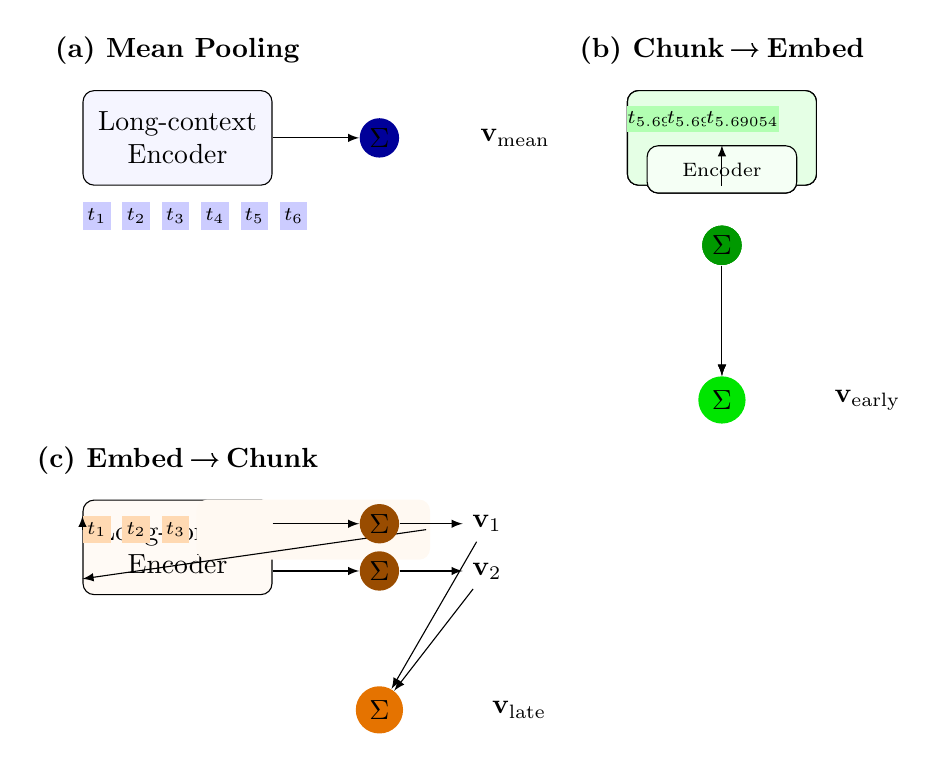
\begin{tikzpicture}[>=latex]

% -----------------------------------------------------
%  (a) MEAN POOLING
% -----------------------------------------------------
\node[draw, rounded corners, minimum height=1.2cm, minimum width=2.4cm,
      align=center, fill=blue!4] (encA) {Long-context\\ Encoder};

% Tokens (a) – show only a few for space
\foreach \i in {1,...,6}{
  \node[fill=blue!20, minimum size=3.5mm, inner sep=0pt,
        below=2mm of encA.south west, anchor=north west,
        xshift={(\i-1)*5mm}] (ta\i) {{\scriptsize $t_{\i}$}};
}

% Mean pooling gadget
\node[circle, fill=blue!60!black, inner sep=0pt, minimum size=5mm,
      right=1.1cm of encA] (meanA) {\(\Sigma\)};

\draw[->] (encA) -- (meanA);

\node[right=0.9cm of meanA, anchor=west] (outA) {\(\mathbf{v}_{\text{mean}}\)};

% Title
\node[above=2mm of encA] {\textbf{(a) Mean Pooling}};

% -----------------------------------------------------
%  (b) CHUNK FIRST, THEN EMBED
% -----------------------------------------------------
% Chunk rectangles
\foreach \i [count=\k from 0] in {1,...,3}{
  \node[draw, fill=green!10, rounded corners,
        minimum height=1.2cm, minimum width=2.4cm,
        right=4.5cm + \k*0cm of encA] (chunk\i) {};

  % Tokens inside each chunk
  \foreach \j in {1,...,3}{
    \pgfmathparse{int((\i-1)*3+\j)}
    \node[fill=green!30, minimum size=3.2mm, inner sep=0pt,
          below=2mm of chunk\i.north west, anchor=north west,
          xshift={(\j-1)*5mm}] (tb\i\j) {{\scriptsize $t_{\pgfmathresult}$}};
  }

  % Encoder inside each chunk
  \node[draw, rounded corners, minimum width=1.9cm,
        minimum height=0.6cm, fill=green!4,
        below=7mm of chunk\i.north] (encb\i) {\scriptsize Encoder};

  \draw[->] (chunk\i) -- (encb\i);

  % CLS / Mean per chunk
  \node[circle, fill=green!60!black, inner sep=0pt,
        minimum size=5mm, below=4mm of encb\i] (poolb\i) {\(\Sigma\)};
}

% Aggregate across chunks
\node[circle, fill=green!90!black, inner sep=0pt,
      minimum size=6mm, below=1.4cm of poolb2] (aggB) {\(\Sigma\)};

\foreach \i in {1,...,3}{
  \draw[->] (poolb\i) -- (aggB);
}

\node[right=1cm of aggB] (outB) {\(\mathbf{v}_{\text{early}}\)};

\node[above=2mm of chunk2] {\textbf{(b) Chunk\,→\,Embed}};

% -----------------------------------------------------
%  (c) LATE CHUNKING
% -----------------------------------------------------
% Encoder (full doc)
\node[draw, rounded corners, minimum height=1.2cm, minimum width=2.4cm,
      align=center, fill=orange!4, below=5.2cm of encA.west, anchor=west] (encC) 
      {Long-context\\ Encoder};

% All tokens (9 for sketch)
\foreach \i in {1,...,9}{
  \node[fill=orange!30, minimum size=3.5mm, inner sep=0pt,
        below=2mm of encC.north west, anchor=north west,
        xshift={(\i-1)*5mm}] (tc\i) {{\scriptsize $t_{\i}$}};
}

% Overlapping windows: window 1 and 2 (semi-transparent)
\begin{scope}[fill=orange!10, rounded corners, draw=orange!70]
  \path ($(tc1.north west)+(-0.5mm,2.0mm)$) rectangle ($(tc6.south east)+(0.5mm,-2.0mm)$);
  \path[fill=orange!5] ($(tc4.north west)+(-0.5mm,2.0mm)$) rectangle ($(tc9.south east)+(0.5mm,-2.0mm)$);
\end{scope}

% Arrows to encoder
\draw[->] (tc1.west) -- ($(encC.west)+(0,0.4)$);
\draw[->] (tc9.east) -- ($(encC.west)-(0,0.4)$);

% Window pooling operations
\node[circle, fill=orange!60!black, inner sep=0pt, minimum size=5mm,
      right=1.1cm of encC, yshift=0.3cm] (poolC1) {\(\Sigma\)};
\node[circle, fill=orange!60!black, inner sep=0pt, minimum size=5mm,
      right=1.1cm of encC, yshift=-0.3cm] (poolC2) {\(\Sigma\)};

\draw[->] ($(encC.east)+(0,0.3)$) -- (poolC1);
\draw[->] ($(encC.east)-(0,0.3)$) -- (poolC2);

% Window vectors
\node[right=0.8cm of poolC1, anchor=west] (vecC1) {\(\mathbf{v}_1\)};
\node[right=0.8cm of poolC2, anchor=west] (vecC2) {\(\mathbf{v}_2\)};

\draw[->] (poolC1) -- (vecC1);
\draw[->] (poolC2) -- (vecC2);

% Final aggregation
\node[circle, fill=orange!90!black, inner sep=0pt,
      minimum size=6mm, below=1.2cm of poolC2] (aggC) {\(\Sigma\)};

\draw[->] (vecC1) -- (aggC);
\draw[->] (vecC2) -- (aggC);

\node[right=1cm of aggC] (outC) {\(\mathbf{v}_{\text{late}}\)};

\node[above=2mm of encC] {\textbf{(c) Embed\,→\,Chunk}};

\end{tikzpicture}
\caption{Three document-level pooling strategies: (a) Mean Pooling applies global averaging over all token embeddings, (b) Chunk-First-Then-Embed splits the document into chunks before encoding, then pools chunk embeddings, (c) Embed-Then-Chunk encodes the full document with a long-context transformer, then applies windowed pooling on the token embeddings before final aggregation.}
\label{fig:pooling-strategies}
\end{figure}

\section{Results}\label{sec:results}

In this section outline your results. At this point, you are just stating the outcome of your analysis. You can highlight important aspects (``we observe a significantly higher value of $x$ over $y$''), but leave interpretation and opinion to the next section. This section absoultely \emph{must} include at least two figures.

\section{Discussion \& Conclusion}\label{sec:conclusion}

Use this section to briefly summarize the entire text. Highlight limitations and problems, but also make clear statements where they are possible and supported by the analysis. 

\newpage

\section*{Contribution Statement}
Explain here, in one sentence per person, what each group member contributed. For example, you could write: Max Mustermann collected and prepared data. Gabi Musterfrau and John Doe performed the data analysis. Jane Doe produced visualizations. All authors will jointly wrote the text of the report. Note that you, as a group, a collectively responsible for the report. Your contributions should be roughly equal in amount and difficulty.

\section*{Notes} 

Your entire report has a \textbf{hard page limit of 4 pages} excluding references and the contribution statement. (I.e. any pages beyond page 4 must only contain the contribution statement and references). Appendices are \emph{not} possible. But you can put additional material, like interactive visualizations or videos, on a githunb repo (use \href{https://github.com/pnkraemer/tueplots}{links} in your pdf to refer to them). Each report has to contain \textbf{at least three plots or visualizations}, and \textbf{cite at least two references}. More details about how to prepare the report, inclucing how to produce plots, cite correctly, and how to ideally structure your github repo, will be discussed in the lecture, where a rubric for the evaluation will also be provided.


\bibliography{bibliography}
\bibliographystyle{icml2025}

\end{document}

% This document was modified from the files available at https://icml.cc/Conferences/2025/AuthorInstructions
% the full copyright notice is available within the file icml2025.sty